\chapter{El microprocesador}\label{chapter:microprocesador}

El \textbf{microprocesador} es un procesador de computadora, donde la lógica del procesamiento de datos y el control
están incluidos en un solo circuito integrado, o en un pequeño número de circuitos integrados. El \textbf{microprocesador}
contiene los circuitos aritméticos, lógicos y de control necesarios para realizar las funciones de la unidad central de
procesamiento  de una computadora. El circuito integrado es capaz de interpretar y ejecutar instrucciones de programa y
realizar operaciones aritméticas. El \textbf{microprocesador} es un circuito integrado digital multipropósito, controlado
por reloj y basado en registros que acepta datos binarios como entrada, los procesa de acuerdo con las instrucciones
almacenadas en su memoria y proporciona resultados (también en forma binaria) como salida. Un \textbf{microprocesador}
hipotético mínimamente funcional podría incluir solo una \textbf{ALU}(\emph{Arithmetic Logic Unit}) y una sección lógica
de control. La \textbf{ALU} realiza sumas, restas y operaciones como \textbf{AND} y \textbf{OR}. Cada operación de la
\textbf{ALU} establece uno o más \emph{flags} en un registro de estados, que indican los resultados de la última operación
(por ejemplo, si el resultado es cero, si es negativo, si hay desbordamiento, etc.). La lógica de control recupera los
código de instrucción desde la memoria e inicia la secuencia de operaciones necesarias parar que la \textbf{ALU} lleve a
cabo la instrucción \brackcite{wikipedia_2022_Microprocesador}.\\ Antes de los microprocesadores las computadoras pequeñas
se construían utilizando  \emph{racks} de placas de circuito con muchos circuitos integrados de mediana y pequeña escala,
generalmente del tipo \textbf{TTL}\emph{(Transistor-Transistor Logic)} \brackcite{wikipedia_2022_ttl}. Los microprocesadores
combinaron esto en uno o unos pocos circuitos integrados a gran escala.\\ El incremento continuo de las capacidades de los
microprocesadores desde  que se empezaron a fabricar ha dejado otras formas de computadoras casi complemtamente obsoletas,
con uno o más microprocesadores usados en todo desde pequeños sistemas embebidos y dispostivos portátiles hasta los enormes
\emph{mainframes} y las supercomputadoras

\section{Surgimiento del microprocesadaor}
Las invenciones a veces ocurren cuando las personas se enfrentan a un problema y luchan por resolverlo. En otras ocasiones, suceden 
cuando las personas adoptan una meta visionaria. La historia de cómo \emph{Ted Hoff} y su equipo de \emph{Intel} inventaron el \textbf
{microprocesador} es un caso de ambos \brackcite{isaacson_2014}. \emph{Hoff}, que había sido un joven profesor en \emph{Stanford}, se
convirtió en el duodécimo empleado de \emph{Intel}, donde fue asignado para trabajar en el diseño de chips. \emph{Hoff} se dió cuenta de que era un
desperdicio y poco elegante diseñar muchos tipos de microchips donde cada uno tuviera una función diferente,  que era lo que \textbf
{Intel} estaba haciendo hasta ahora. Llegaría una empresa y le pediría que construyera un \textbf{microchip} diseñado para realizar una tarea
específica. \emph{Hoff} imaginó, al igual que \emph{Noyce} y otros, un enfoque alternativo: crear un \textbf{chip} de propósito general que pudiera
ser instruido o programado para realizar una variedad de aplicaciones diferentes según se desee. En otras palabras, una computadora de propósito
general en un \textbf{chip}. Esta visión coincidió con un problema que se planteó a \emph{Intel} en el verano de 1969. Una empresa japonesa llamada \emph
{Busicom} estaba planeando una nueva y poderosa calculadora de escritorio : la \textbf{Busicom 141-PF}, y había elaborado especificaciones para
doce microchips de propósito especial para diseñar 12 chips personalizados para su nueva calculadora de impresión (diferentes para
manejar pantalla, cálculos, memoria, etc.) que quería que \emph{Intel} construyera. \emph{Intel} estuvo de acuerdo y se fijó un precio. \emph{Noyce} le
pidió a \emph{Hoff} que supervisara el proyecto. La cantidad de chips y su complejidad fue mucho mayor de lo que esperaba, por lo que no
había forma de que \emph{Intel} pudidiera construirlos al precio acordado. \emph{Intel} se propuso diseñar un solo \textbf{chip} lógico
que pudiera realizar casi todas las tareas que quería \emph{Busicom}. Para empeorar las cosas,  la creciente popularidad de la calculadora
de bolsillo de \emph{Jack Kilby} estaba obligando a \emph{Busicom} a reducir aún más su precio. \emph{Noyce} le dijo a \emph{Intel} que lo intentara y  tuvo que
convencer a Grove del proyecto antes de venderle la idea a \emph{Busicom}. En septiembre de 1969, \emph{Intel} y su colega \emph{Stan Mazor} habían esbozado
la arquitectura de un \textbf{chip} lógico de uso general que podía seguir instrucciones de programación. Sería capaz de hacer el trabajo de
nueve de los doce chips que había solicitado \emph{Busicom}. Se diseñaron un conjunto cuatro chips conocido como \textbf{MCS-4}. Incluía un \textbf{chip} de
unidad de procesamiento central (\textbf{CPU}), el \textbf{4004}, así como un \textbf{chip} de memoria de solo lectura (\textbf{ROM}) compatible para los programas de
aplicaciones personalizadas, un \textbf{chip} de memoria de acceso aleatorio (\textbf{RAM}) para procesar datos, y un \textbf{chip} de registro para el puerto
de entrada/salida (E/S). Cuando llegó el momento de renegociar el precio, \emph{Intel} hizo una recomendación fundamental a \emph{Noyce}, que ayudó
a crear un gran mercado para los chips de uso general y aseguró que \emph{Intel} seguiría siendo un impulsor de la era digital. A cambio de
darle a \emph{Busicom} un buen precio, \emph{Noyce} insistió en que \emph{Intel} retuviera los derechos del nuevo \textbf{chip} y se le permitiera licenciarlo a otras 
compañías para fines distintos a la fabricación de una calculadora. Debido a que era esencialmente un procesador de computadora en un \textbf{chip},
el nuevo dispositivo se denominó \textbf{microprocesador}. En noviembre de 1971 \emph{Intel} dio a conocer el producto, el \textbf{Intel 4004}, al público.
Este tenía un precio de salida de \$200 \brackcite{intel_4004, wikipedia_2022_Microprocesador,campbell-kelly_garcia-swartz_2015,isaacson_2014}.

\begin{figure}[htb]
	\centering
	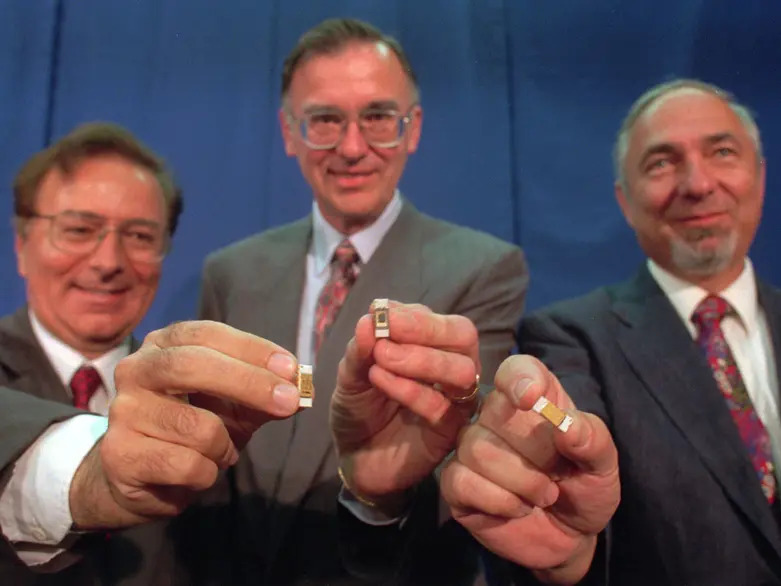
\includegraphics[scale = 0.25]{Graphics/faggin_hoff_mazor_-4004.jpg}
	\caption{Desde la izquierda, \emph{Federico Faggin}, \emph{Ted Hoff} y \emph{Stanley Mazor} con procesadores \textbf{Intel 4004}}
	\label{fig:10}
\end{figure}

\subsection{Intel 4004}
Este revolucionario \textbf{microprocesador}, del tamaño de la uña del dedo meñique, entregaba la misma potencia de cómputo que la primera
computadora electrónica construida en 1946, que llenó una habitación entera. El primer \textbf{microprocesador} \textbf{Intel 4004} se
fabricó en obleas de dos pulgadas, en comparación con las obleas de 12 pulgadas que se utilizan habitualmente en los productos actuales.
El \textbf {microprocesador} \textbf{Intel 4004} es único en el sentido de que es uno de los diseños de \textbf{microprocesador} más
pequeños que alguna vez entró en producción comercial. El \textbf{4004}  era un \textbf{microprocesador} de \textbf{4-bits}, alcanzaba una máxima
velocida de reloj 740 kHz. El ancho de línea del circuito del \textbf{microprocesador} \textbf{Intel 4004} era de 10 micrones o 10 000
nanómetros. En 1971 el \textbf{Intel 4004} contenía 2300 transistores Para el 2010, un procesador \textbf{Intel Core} con matriz de procesamiento
de 32 nm y tecnología de \textbf{silicio} de puerta metálica de alta k de segunda generación contenía  560 millones de transistores. En comparación,
un cabello humano promedio tiene 100,000 nanómetros de ancho \brackcite{intel_4004,wikipedia_2022_intel_4004}.      

\begin{figure}[htb]
	\centering
	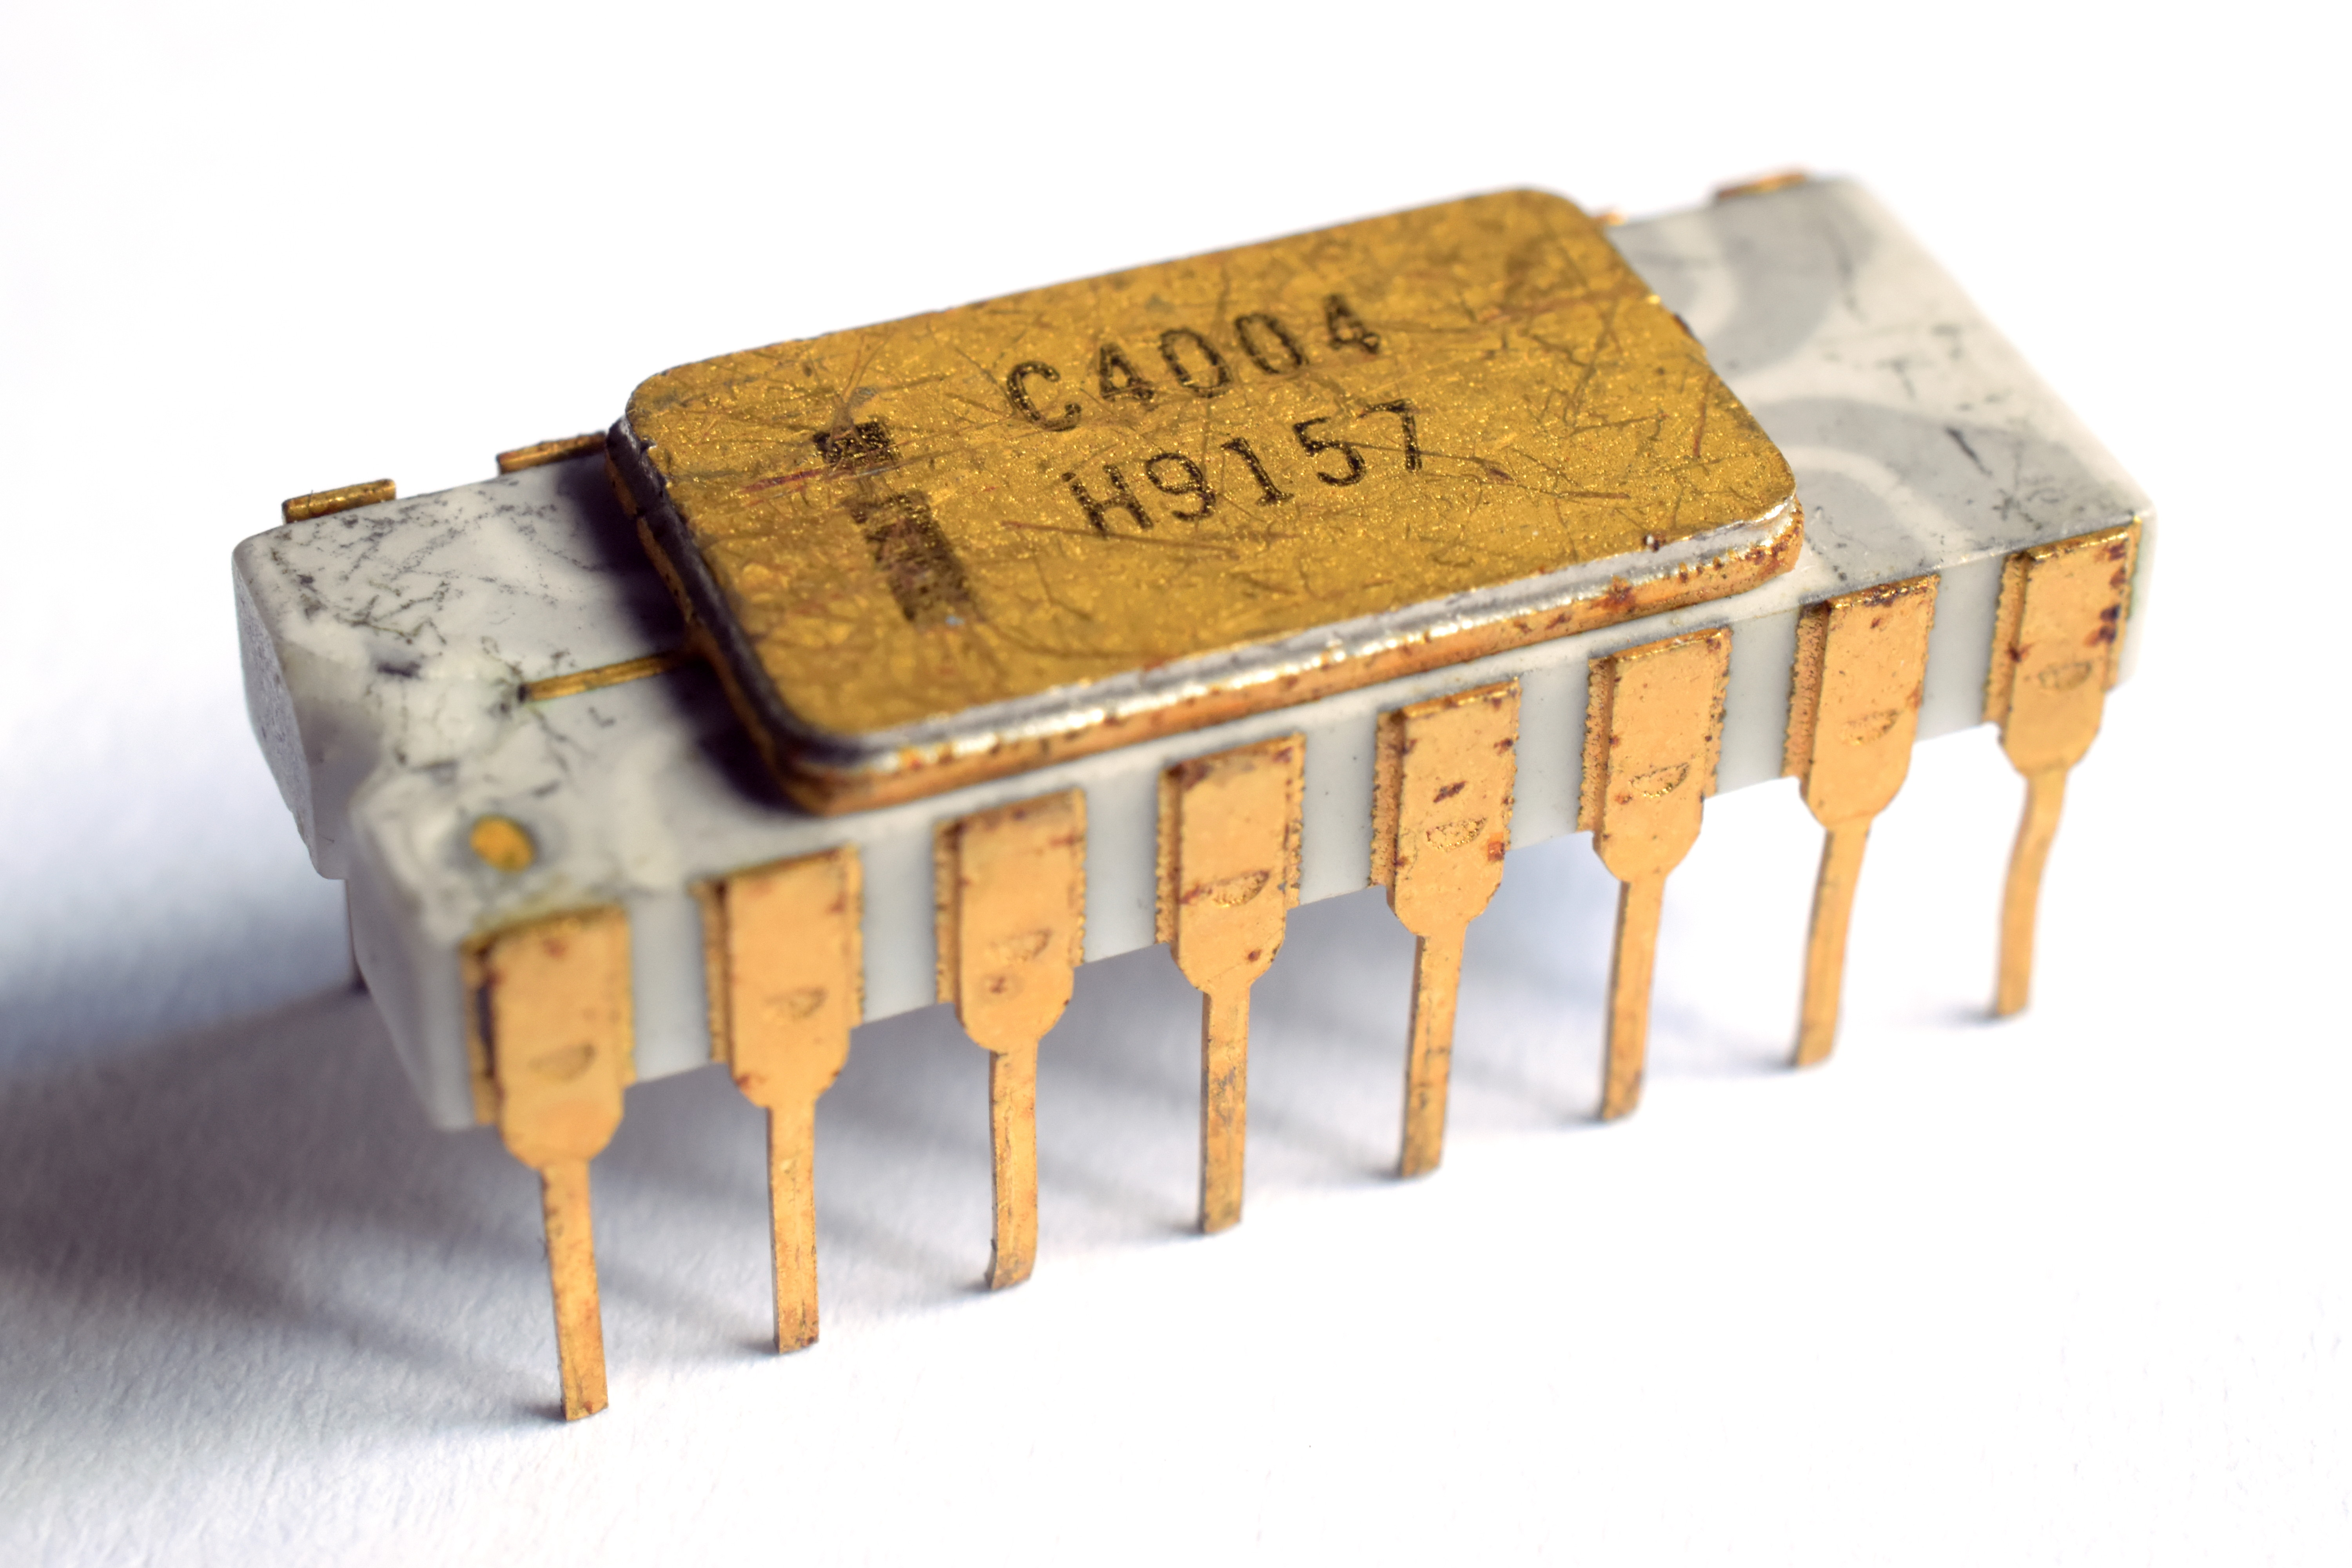
\includegraphics[scale = 0.15]{Graphics/Intel_C4004.jpg}
	\caption{Primer \textbf{microprocesador}: \textbf{Intel 4004}}
	\label{fig:12}
\end{figure}


\section{El arribo del primer microprocesador de 8-bits}
El \textbf{Intel 4004} fue seguido en 1972 por el \textbf{Intel 8008}, el primer \textbf{microprocesador} de 8 bits del mundo.
Sin embargo, el \textbf{8008} no fue una extensión del diseño del \textbf{4004}, sino la culminación de un proyecto de diseño separado
en \emph{Intel}, que surgió de un contrato con \emph{Computer Terminals Corporation}(\textbf{CTC}), por un \textbf{chip} para
una terminal que estaban diseñando: el \textbf{Datapoint 2200}, los aspectos fundamentales del diseño no provinieron de \emph{Intel}
sino de \textbf{CTC}. El \textbf{8008} salió con 3.500 transistores, tenía un bus de datos de 8 bits y un bus de direcciones de 14 bits. Este
\textbf{micoprocesador} fue la base del famoso kit de computadora "Mark-8" \brackcite{wikipedia_2022_intel_8008, campbell-kelly_garcia-swartz_2015}.

\begin{figure}[htb]
	\centering
	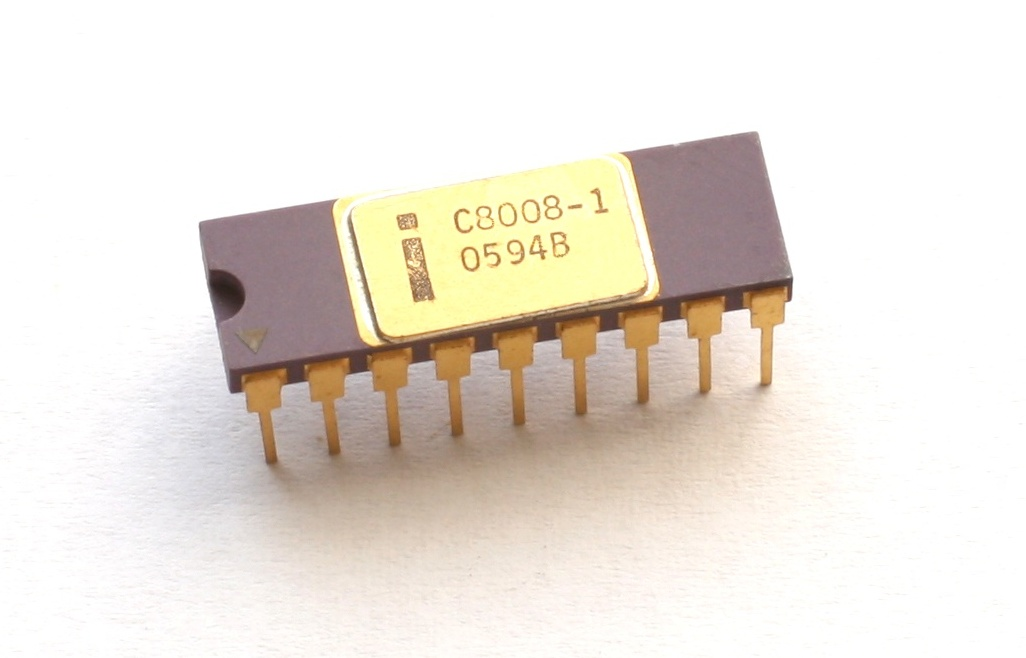
\includegraphics[scale = 0.15]{Graphics/Intel_C8008-1.jpg}
	\caption{\textbf{Microprocesador}  \textbf{Intel 8008}}
	\label{fig:13}
\end{figure}

\subsection{8080}
El Intel \textbf{8080} es el segundo \textbf{microprocesador} de 8 bits diseñado y fabricado por Intel. Apareció por primera vez en abril de 1974 y es una variante ampliada y mejorada
del diseño anterior del \textbf{8008}, aunque sin compatibilidad binaria. La velocidad de reloj o límite de frecuencia especificado inicialmente era de 2 MHz, con instrucciones
comunes que usaban 4, 5, 7, 10 o 11 ciclos. Como resultado, el procesador podía ejecutar varios cientos de miles de instrucciones por segundo. Federico Faggin lo concibió 
y diseñó utilizando MOS de canal N de alto voltaje.

\begin{figure}[htb]
	\centering
	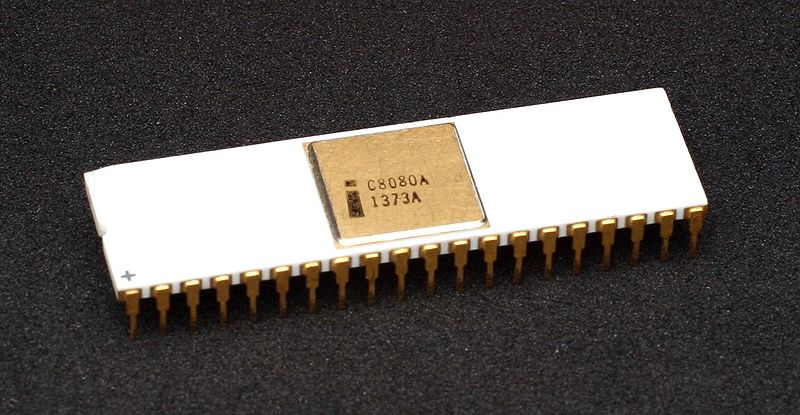
\includegraphics[scale = 0.2]{Graphics/8080_microprocessorr.jpg}
	\caption{\textbf{Microprocesador} \textbf{Intel 8080}}
	\label{fig:14}
\end{figure}

\section{El arribo de los 16 bits}

El primer \textbf{microprocesador} multichip de 16 bits fue el \textbf{IMP-16} de \emph{National Semiconductor}, presentado a principios de 1973. Una versión de 8 bits del conjunto de 
chips se introdujo en 1974 como \textbf{IMP-8}. Durante el mismo año, \emph{National} presentó el primer \textbf{microprocesador} de un solo \textbf{chip} de 16 bits, el \textbf{PACE},
seguido de una versión NMOS, el \textbf{INS8900}. El primer \textbf{microprocesador} de 16 bits de un solo chip fue el TMS 9900 de \emph{Texas Instruments}, presentado en 1976, que
también era compatible con su línea de minicomputadoras \textbf{TI-990}. \emph{Intel} produjo su primer procesador de 16 bits, el \textbf{8086}, en 1978. Era compatible con el \textbf{8080}
y el \textbf{8085} (un derivado del \textbf{8080}) \brackcite{wikipedia_2022_Microprocesador,staff_2021_microprocessor}.

\begin{figure}[htb]
	\centering
	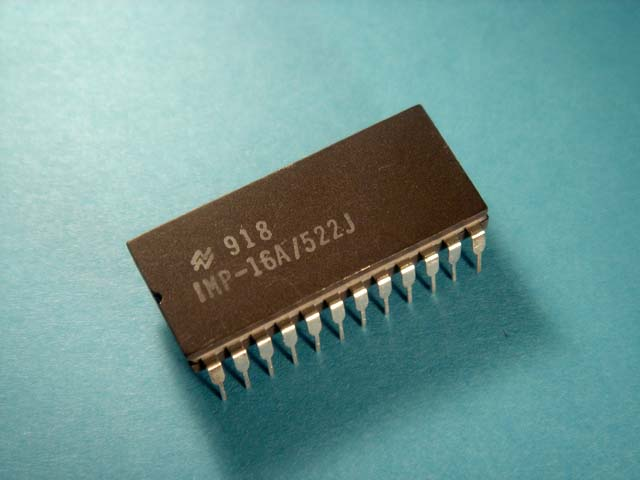
\includegraphics[scale = 0.2]{Graphics/NSIMP-16A.jpg}
	\caption{\textbf{Microprocesador} \textbf{IMP-16}}
	\label{fig:15}
\end{figure}

\section{8086: El comienzo de x86}
El primer procesador de 16 bits de \emph{Intel} fue el \textbf{8086}, que ayudó a mejorar considerablemente el rendimiento en comparación con los diseños anteriores.
Este \textbf{microprocesador} utilizaba la misma microarquitectura que los microprocesadores de 8 bits de Intel (\textbf{8008}, \textbf{8080} y \textbf{8085}). Esto permitió
que los programas en lenguaje ensamblador escritos en 8 bits migraran sin problemas. El \textbf{8086} no solo tenía una frecuencia más alta que la \textbf{8088}, sino que
también empleaba un bus de datos externo de 16 bits y una cola de precarga de 6 bytes más larga. También podía ejecutar tareas de 16 bits (aunque la mayoría del \emph{software} 
en ese momento estaba diseñado para procesadores de 8 bits). El bus de direcciones se amplió a 20 bits, lo que permitió al \textbf{8086} acceder a hasta 1 MB de memoria y,
por lo tanto, aumentar el rendimiento. El \textbf{8086} también se convirtió en el primer procesador x86 y utilizó la primera revisión del x86 ISA \brackcite{wikipedia_2022_x86_ISA},
en el que se han basado casi todos los procesadores creados por \emph{AMD} o \emph{Intel} desde la introducción del \textbf{8086} \brackcite{wikipedia_2022_Microprocesador,
sexton_2018_history_intel_cpus, wikipedia_2022_intel_8086}.

\begin{figure}[htb]
	\centering
	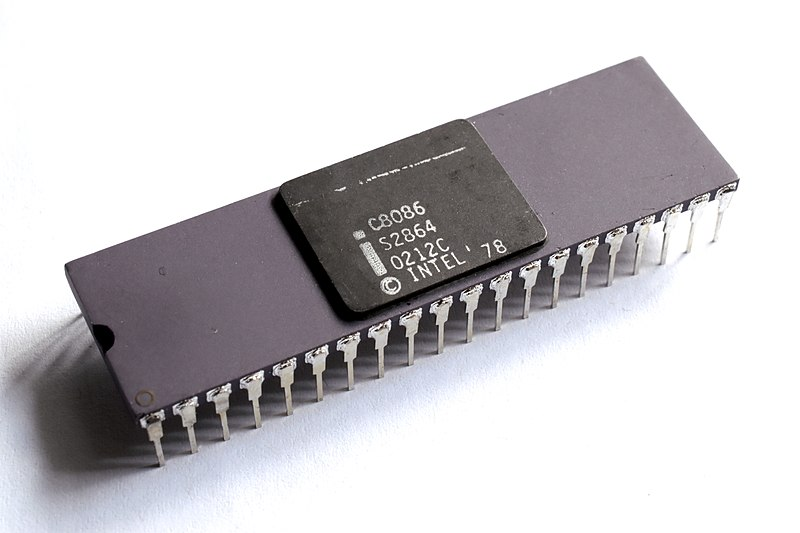
\includegraphics[scale = 0.2]{Graphics/Intel_C8086.jpg}
	\caption{\textbf{Intel 8086}}
	\label{fig:16}
\end{figure}

\section{El arribo de los 32 bits}

% En 1968, Vic Poor y Harry Pyle de CTC 
% desarrollaron el diseño original para el conjunto de instrucciones y el funcionamiento del procesador. En 1969, CTC contrató a dos empresas, Intel y Texas Instruments, para 
% realizar una implementación de un solo chip, conocida como CTC 1201. A fines de 1970 o principios de 1971, TI se retiró al no poder fabricar una pieza confiable. 
% En 1970, con Intel aún por entregar la parte, CTC optó por usar su propia implementación en el Datapoint 2200, usando en su lugar la lógica TTL tradicional 
% (por lo tanto, la primera máquina que ejecutó el "código 8008" no era de hecho un microprocesador y se entregó el año anterior). La versión de Intel del microprocesador 
% 1201 llegó a fines de 1971, pero fue demasiado tarde, lenta y requirió una cantidad de chips de soporte adicionales. CTC no tenía interés en usarlo. CTC había contratado
% originalmente a Intel por el chip y les habría debido 50 000 dólares estadounidenses (equivalente a 334 552 dólares en 2021) por su trabajo de diseño.[43] 
% Para evitar pagar por un chip que no querían (y no podían usar), CTC liberó a Intel de su contrato y les permitió el uso gratuito del diseño.[43] Intel 
% lo comercializó como 8008 en abril de 1972, como el primer microprocesador de 8 bits del mundo. Fue la base del famoso kit de computadora "Mark-8". 

% En 1973, Intel lanzó el primer procesador de 8 bits ampliamente utilizado, llamado Intel 8008. El 8008 salió con 3.500 transistores. . En este sistema, el bus de datos y 
% las direcciones eran unidades de 8 bits. El Intel 4004 fue seguido en 1972 por el Intel 8008, el primer microprocesador de 8 bits del mundo. Sin embargo, el 8008 no fue 
% una extensión del diseño del 4004, sino la culminación de un proyecto de diseño separado en Intel, que surgió de un contrato con Computer Terminals Corporation, de San Antonio TX, 
% por un chip para una terminal que estaban diseñando, [42] el Datapoint 2200: los aspectos fundamentales del diseño no provinieron de Intel sino de CTC.



 % Pronto surgió un desafío. “Cuanto más aprendía sobre este diseño, más me 
% preocupaba que Intel pudiera haber emprendido más de lo que estaba preparado para entregar”, recordó Hoff. "La cantidad de chips y su 
% complejidad fue mucho mayor de lo que esperaba". No había forma de que Intel pudiera construirlos al precio acordado. .
% Hoff propuso que Intel diseñara un solo chip lógico que pudiera realizar casi todas las tareas que quería Busicom

% “Bueno, si hay algo que se te ocurra para simplificar el diseño, ¿por qué no lo persigues?”, sugirió Noyce.
% . 
% “Sé que esto se puede hacer”, dijo sobre el chip de propósito general. “Se puede hacer para emular una computadora”. 
% Noyce le dijo que lo intentara. 
% Antes de que pudieran vender la idea a Busicom, Noyce se dio cuenta de que tenía que convencer a alguien que podría oponerse 
% aún más: Andy Grove, quien nominalmente trabajaba para él. Parte de lo que Grove vio como su mandato era mantener a Intel enfocado.

% Noyce diría que sí a casi cualquier cosa; El trabajo de Grove era decir que no. Cuando Noyce se acercó al espacio de trabajo de Grove y se 
% sentó en la esquina de su escritorio, Grove se puso inmediatamente en guardia. Sabía que el esfuerzo de Noyce por parecer indiferente era una 
% señal de que algo estaba pasando. “Estamos comenzando otro proyecto”, dijo Noyce, fingiendo reír.53 La primera reacción de Grove fue decirle a 
% Noyce que estaba loco. Intel era una empresa incipiente que todavía luchaba por fabricar sus chips de memoria y no necesitaba distracciones. Pero 
% después de escuchar a Noyce describir la idea de Hoff, Grove se dio cuenta de que la resistencia probablemente estaba mal y definitivamente era inútil.
% En septiembre de 1969, Hoff y su colega Stan Mazor habían esbozado la arquitectura de un chip lógico de uso general que podía seguir instrucciones de programación. 
%  Noyce y Hoff presentaron la opción a los ejecutivos de Busicom, 
% quienes acordaron que era el mejor enfoque.

% .  Fue un punto de negociación que Bill Gates y Microsoft emularían con IBM una década después. 
% A cambio de darle a Busicom un buen precio, Noyce insistió en que Intel retuviera los derechos del nuevo chip y se le permitiera licenciarlo a otras compañías 
% para fines distintos a la fabricación de una calculadora. 

% Se dio cuenta de que un chip que pudiera programarse para realizar cualquier función lógica se convertiría en un componente estándar en los dispositivos electrónicos, 
% de la misma manera que las piezas de madera de dos por cuatro eran un componente estándar en la construcción de casas.
% Reemplazaría los chips personalizados, lo que significaba que podría fabricarse a granel y, por lo tanto, su precio disminuiría continuamente. También marcaría el 
% comienzo de un cambio más sutil en la industria electrónica: la importancia de los ingenieros de hardware, que diseñaron la 

% ubicación de los componentes en una placa de circuito, comenzó a ser suplantada por una nueva generación, los ingenieros de software, cuyo trabajo era programar 
% Debido a que era esencialmente un procesador de computadora en un chip, el nuevo dispositivo se denominó microprocesador. En noviembre de 1971 Intel dio a conocer 
% el producto, el Intel 4004, al público. Sacó anuncios en revistas especializadas que anunciaban “una nueva era de electrónica integrada: ¡una computadora microprogramable en 
% un chip!” Tenía un precio de \$ 200 y los pedidos, así como miles de solicitudes del manual, comenzaron a llegar. Noyce asistía a una exhibición de computadoras en 
% Las Vegas el día del anuncio y estaba emocionado de ver a los clientes potenciales abarrotar la suite de Intel.

% 1969: La misión
% En 1969, Nippon Calculating Machine Corporation se acercó a Intel para diseñar 12 chips personalizados para su nueva calculadora de impresión Busicom 141-PF*. 
% Los ingenieros de Intel sugirieron una familia de solo cuatro chips, incluido uno que podría programarse para su uso en una variedad de productos, poniendo en 
% marcha una hazaña de ingeniería que alteró drásticamente el curso de la electrónica.


% 1971: era de la electrónica integrada
% Intel compró los derechos de Nippon Calculating Machine Corporation y lanzó el procesador Intel® 4004 y su conjunto de chips con un anuncio en la edición del 15 de noviembre 
% de 1971 de Electronic News: "Anunciando una nueva era en la electrónica integrada".
% Fue entonces cuando Intel® 4004 se convirtió en el primer procesador programable de uso general del mercado: un "bloque de construcción" que los ingenieros podían comprar y 
% luego personalizar con software para realizar diferentes funciones en una amplia variedad de dispositivos electrónicos.

% oderosamente pequeño, incluso en 1971
% Este microprocesador revolucionario, del tamaño de la uña del dedo meñique, entregaba la misma potencia de cómputo que la primera computadora electrónica construida en 
% 1946, que llenó una habitación entera.



